\section{'DHL Express Mobile' Application Analysis by Rafael}

The application that was analyzed in this chapter had the name 'DHL'.
The application was found on \href{https://koodous.com/apks/38ff459a46e9ea6d63a83c1eddb640626fef562cd1bcb0ab3823c4770d07d0fb}{Koodous} with the version \texttt{1.0} and package name \texttt{com.ru.dhl}, the size was \texttt{2.7 MB}.
The same package name did not exist on the Google Play Store. However, an application with the same icon was found \href{https://play.google.com/store/apps/details?id=com.dhl.exp.dhlmobile}{here}. It has the version \texttt{2.7.0}, package name \texttt{com.dhl.exp.dhlmobile} and a size of \texttt{25 MB}.

The application found on Koodous and the application found on the Google Play Store will hereinafter be referred to as 'Malicious application' and 'Original application' respectively.

\subsection{VirusTotal summary}

The malicious application was uploaded to VirusTotal to get a first impression of its capabilities.
VirusTotal indicated that the malicious application was marked by 33/63 security vendors as malicious, 
and that the original application was marked by 0/60 security vendors as malicious.

The malicious application was primarily marked as a Banker\footnote{A banker generally is an application that attempts to steal banking information in order to steal the user's money.\label{footnote-banker}}. 
If it was not marked as a banker it was either marked as a Trojan\footnote{A Trojan (or 'Trojan Horse malware') is a blanket term for malicious software that disguises itself as a harmless application\label{footnote-trojan}} or a non repeating name.
This was the full list


\begin{tabular}{ |l|l| }
    \hline
    \textbf{Vendor} & \textbf{Detection} \\
    
    \hline
        Ad-Aware    &   Trojan.GenericKD.37488882 \\
    \hline
        Alibaba     &   TrojanSpy:Android/Banker.66c12705 \\
    \hline
        Antiy-AVL   &   Trojan/Generic.ASMalwAD.5B \\
    \hline
        Arcabit     &   Trojan.Generic.D23C08F2 \\
    \hline
        Avast-Mobile    &   APK:RepSandbox [Trj] \\
    \hline
        Avira (no cloud)    &   ANDROID/Spy.Banker.YD.Gen \\
    \hline
        BitDefender     &   Trojan.GenericKD.37488882 \\
    \hline
        BitDefenderFalx     &   Android.Trojan.Banker.WS \\
    \hline
        CAT-QuickHeal   &   Android.AbereBot.Af9d \\
    \hline
        Cynet   &   Malicious (score: 99) \\
    \hline
        DrWeb   &   Android.BankBot.852.origin \\
    \hline
        Emsisoft    &   Trojan.GenericKD.37488882 (B) \\
    \hline
        eScan   &   Trojan.GenericKD.37488882 \\
    \hline
        ESET-NOD32  &   A Variant Of Android/Spy.Banker.AZU \\
    \hline
        F-Secure    &   Malware.ANDROID/Spy.Banker.YD.Gen \\
    \hline
        FireEye     &   Trojan.GenericKD.37488882 \\
    \hline
        Fortinet    &   Android/AbereBot.A!tr \\
    \hline
        GData   &   Trojan.GenericKD.37488882 \\
    \hline
        Gridinsoft  &   Trojan.U.Banker.oa \\
    \hline
        Ikarus  &   Trojan.AndroidOS.Banker \\
    \hline
        K7GW    &   Spyware ( 005817811 ) \\
    \hline
        Kaspersky   &   HEUR:Trojan-Banker.AndroidOS.AbereBot.a \\
    \hline
        Kingsoft    &   Android.Troj.tn-banker.azu.(kcloud) \\
    \hline
        Lionic  &   Trojan.AndroidOS.AbereBot.C!c \\
    \hline
        MAX     &   Malware (ai Score=100) \\
    \hline
        McAfee  &   Artemis!4778ACA48D17 \\
    \hline
        McAfee-GW-Edition   &   Artemis!Trojan \\
    \hline
        Microsoft   &   TrojanSpy:AndroidOS/Banker.GV!MTB \\
    \hline
        Symantec    &   Trojan.Gen.MBT \\
    \hline
        Symantec Mobile Insight     &   AppRisk:Generisk \\
    \hline
        Tencent     &   A.privacy.AnubisTrojanBanking \\
    \hline
        Trustlook   &   Android.Malware.Trojan \\
    \hline
        ZoneAlarm by Check Point    &   HEUR:Trojan-Banker.AndroidOS.AbereBot.a \\
    \hline
\end{tabular}
\subsubsection{Permission requests}

This chapter will describe the permissions requested by the malicious and original application.

\subsubsubsection{Malicious application}
The malicious application requested the following permissions:

\texttt{android.permission.ACCESS\_NETWORK\_STATE}
\newline \texttt{android.permission.ACCESS\_WIFI\_STATE}
\newline \texttt{android.permission.CALL\_PHONE}
\newline \texttt{android.permission.CHANGE\_WIFI\_STATE}
\newline \texttt{android.permission.FOREGROUND\_SERVICE}
\newline \texttt{android.permission.INTERNET}
\newline \texttt{android.permission.MODIFY\_AUDIO\_SETTINGS}
\newline \texttt{android.permission.READ\_CALL\_LOG}
\newline \texttt{android.permission.READ\_CONTACTS}
\newline \texttt{android.permission.READ\_PHONE\_STATE}
\newline \texttt{android.permission.READ\_PRIVILEGED\_PHONE\_STATE}
\newline \texttt{android.permission.READ\_SMS}
\newline \texttt{android.permission.RECEIVE\_BOOT\_COMPLETED}
\newline \texttt{android.permission.RECEIVE\_SMS}
\newline \texttt{android.permission.REQUEST\_DELETE\_PACKAGES}
\newline \texttt{android.permission.REQUEST\_IGNORE\_BATTERY\_OPTIMIZATIONS}
\newline \texttt{android.permission.SEND\_SMS}
\newline \texttt{android.permission.SHUTDOWN}
\newline \texttt{android.permission.UPDATE\_DEVICE\_STATS}
\newline \texttt{android.permission.WAKE\_LOCK}
\newline \texttt{android.permission.WRITE\_CALL\_LOG}
\newline \texttt{android.permission.WRITE\_CONTACTS}

There were definitely were some interesting permissions requested, for example the DHL application would under no circumstances need to read the contacts.

\newpage
\subsubsubsection{Original application}
The original application requested the following permissions:

\texttt{android.permission.CALL\_PHONE}
\newline \texttt{android.permission.FLASHLIGHT}
\newline \texttt{android.permission.READ\_APP\_BADGE}
\newline \texttt{android.permission.READ\_EXTERNAL\_STORAGE}
\newline \texttt{android.permission.READ\_PHONE\_STATE}
\newline \texttt{android.permission.USE\_FINGERPRINT}
\newline \texttt{android.permission.WRITE\_EXTERNAL\_STORAGE}
\newline \texttt{com.anddoes.launcher.permission.UPDATE\_COUNT}
\newline \texttt{com.dhl.exp.dhlmobile.permission.C2D\_MESSAGE}
\newline \texttt{com.google.android.c2dm.permission.RECEIVE}
\newline \texttt{com.htc.launcher.permission.READ\_SETTINGS}
\newline \texttt{com.htc.launcher.permission.UPDATE\_SHORTCUT}
\newline \texttt{com.huawei.android.launcher.permission.CHANGE\_BADGE}
\newline \texttt{com.huawei.android.launcher.permission.READ\_SETTINGS}
\newline \texttt{com.huawei.android.launcher.permission.WRITE\_SETTINGS}
\newline \texttt{com.majeur.launcher.permission.UPDATE\_BADGE}
\newline \texttt{com.oppo.launcher.permission.READ\_SETTINGS}
\newline \texttt{com.oppo.launcher.permission.WRITE\_SETTINGS}
\newline \texttt{com.sec.android.provider.badge.permission.READ}
\newline \texttt{com.sec.android.provider.badge.permission.WRITE}
\newline \texttt{com.sonyericsson.home.permission.BROADCAST\_BADGE}
\newline \texttt{com.sonymobile.home.permission.PROVIDER\_INSERT\_BADGE}
\newline \texttt{me.everything.badger.permission.BADGE\_COUNT\_READ}
\newline \texttt{me.everything.badger.permission.BADGE\_COUNT\_WRITE}

It was quite interesting to see how little of the permissions were common between the malicious and original application.
This indicated that the malicious application was no repackaged.
\subsection{Behavior analysis}

As soon as the application was installed it would constantly give a popup telling the user to enable Chrome. 
It also would constantly open a window showing the user how to "enable Chrome". 
If the user tried to force the app to close via these settings it would not work. 
The app would constantly open and force the user to enable the app until it was either uninstalled or enabled.
 
Touching the popup would redirect the user to the Accessibility settings. 
In this menu it would be possible to enable the malicious app. 
What it enabled would not have been shown on these settings.

If the user enabled this setting the application would disappear from the main menu and silently run in the background. 
According to the phone the app would take a lot of battery life, because it would constantly give popups asking to close background applications to save battery power. 
These popups would however be instantly closed by the application.

The only way the user would be able to find this app would be in the application settings. 
Any attempts from the user to remove the app at this stage would be thwarted by the app.
This is shown on figure \ref{tim-appbehavior}

\begin{figure}[H]
    \centering
    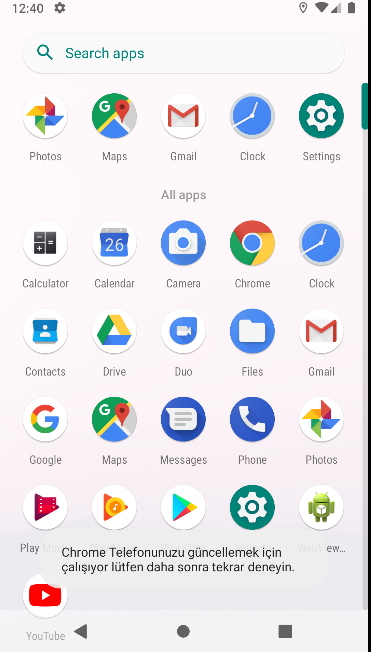
\includegraphics[width=4cm, height=15cm, keepaspectratio]{behaviorimg.png}
    \caption{app booting you from application settings}
    \label{tim-appbehavior}
\end{figure}

The message that the user would have been met with when trying to edit the application settings of the malicious chrome app translated to: 
Chrome is working to update your phone please try again later.

According to the translater this was Turkish hinting that this app might have been made by a Turkish developer.
If the application has reached this stage it would be impossible to remove it from a normal phone.

\subsection{Network analysis}

Analysing the network of the application proved to be a difficult task. 
In order to only retrieve the network traffic from the android emulator Mitmproxy was used.
Mitemproxy had an issue with the Android emulator where it would constantly fail the TLS handshake. 
This made following the new connections hard. 
In order to properly retrieve the all the in-and outgoing traffic \href{https://github.com/shroudedcode/apk-mitm}{apk-mitm} was used.



\subsubsection{HTTP proxy analysis}

Mitmproxy was able to detect an incoming POST request to an outside IP. 
The POST request would connect with the IP address 172.67.131.170 as seen on figure \ref{tim-mitmrequest}.

\begin{figure}[H]
    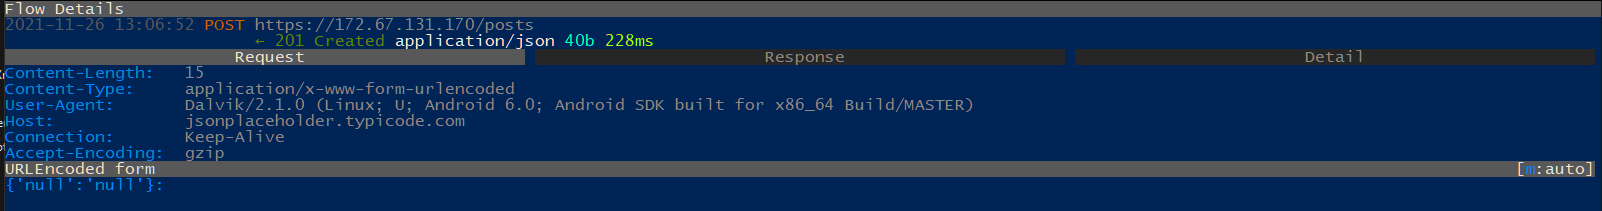
\includegraphics[width=1\textwidth]{mitmreq.png}
    \caption{IP found with mitm}
    \label{tim-mitmrequest}
\end{figure}

\begin{figure}[H]
    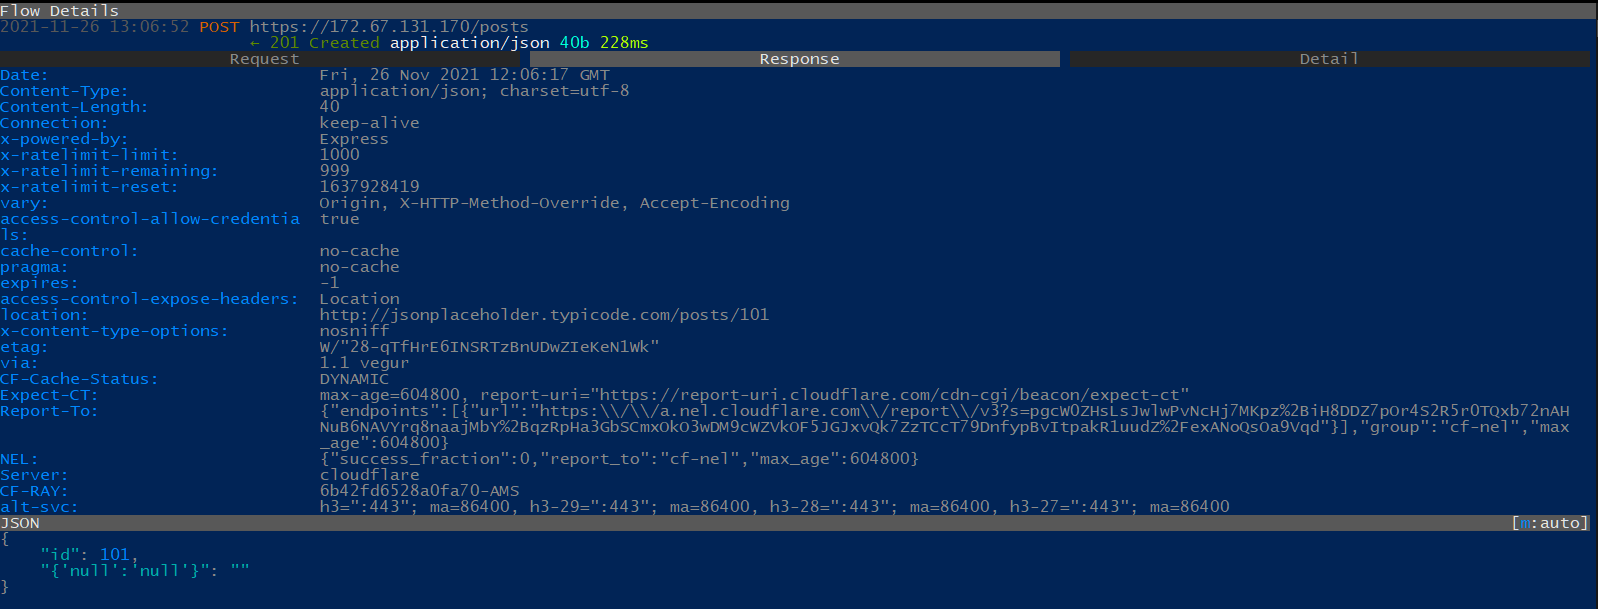
\includegraphics[width=1\textwidth]{networkresponse.png}
    \caption{Response given to the request}
    \label{tim-mitmresponse}
\end{figure}

The POST request contained a JSON file which had an ID with two values. 
The two values however were both null as shown on figure \ref{tim-mitmresponse}.
This was most likely due to an error in the application. 
Also shown on this figure is site that would be sent to.
This site is an online JSON placeholder site.
Any other requests that Mitmproxy picked up were just the expected connections done by google.

\begin{figure}[H]
    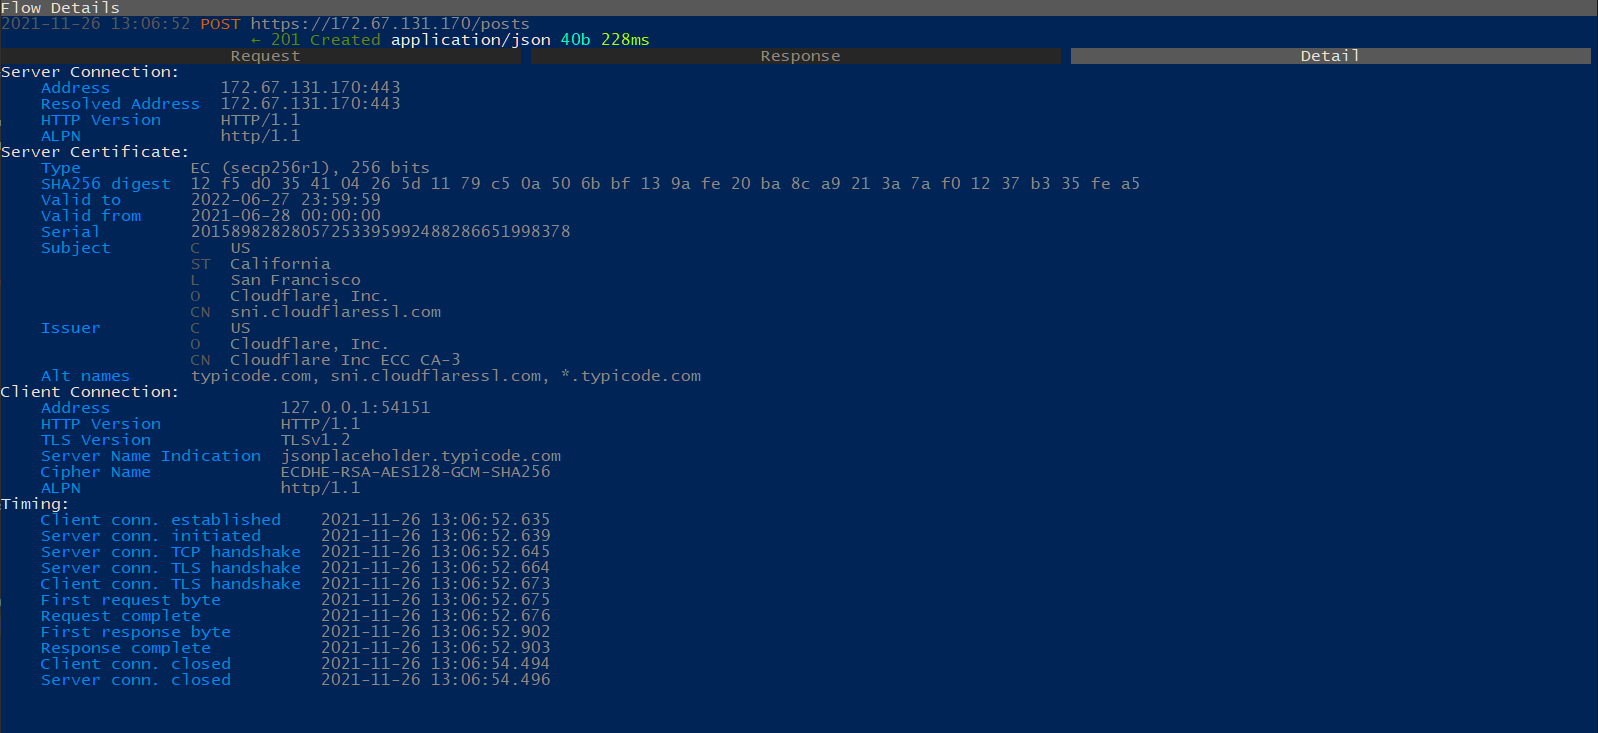
\includegraphics[width=1\textwidth]{networkdetail.png}
    \caption{Details about the connection}
    \label{tim-mitmdetail}
\end{figure}

\subsubsection{Reconnaissance}

A short Reconnaissance was done on the IP address, Mitmproxy had noted it was an Cloudflare connection.
\href{https://www.shodan.io/host/172.67.131.170}{Shodan} backed this showing that it was indeed owned by Cloudflare, Inc.
There was not much else to go on except for that one connection so company that built the app made sure to cover their tracks.

\subsection{Code analysis}

The malicious code was successfully decompiled using JadX, there were quite a lot of elements it was not able to decompile.
However, it seemed like the most important parts were intact. 
The code was obfuscated. The connection between classes was impossible to determine.
However, there were still a lot of useful strings and android interactions.

One of the interesting strings existed in two files, \texttt{sources/d/e/a/b.java} and \texttt{sources/d/c/a/b/a.java}.
The strings contained the domain that requests were being sent to, \texttt{https://api.telegram.org/bot}.
This indicated that the application really was making requests to Telegram.

There was a file that was a lot more interesting, however, \texttt{sources/d/e/a/e.java}.
This file contained a long list of package names, which on a first quick glance looked like package names for popular crypto banking applications.
After some investigating it not only contained crypto banking applications but also regular banking applications and email clients.
It even included Dutch banks such as IGN, ABN AMRO and a few others. 

A list of all the applications in the list can be found in Table \ref{rafael-hackeableapps} included at the end of this section.
Some further investigation indicated that the application was attempting to steal data from these applications and send it somewhere.
It can be assumed that it again sends the data to telegram. However, it was near impossible to find in the code whether this was actually the case.

\newpage
    \begin{longtblr}[
        caption = {All applications that can be hacked},
        label = {rafael-hackeableapps}
    ]{
        colspec = {|l|l|},
        rowhead = 1,
        hlines
    }
    \textbf{Google Play Store application}                & \textbf{Package name}                      \\
                                                          & io.hotbit.shouy                            \\
                                                          & localbitcoin                               \\
                                                          & pl.ideabank.mobilebanking                  \\
    ABN AMRO                                              & com.abnamro.nl.mobile.payments             \\
    Albaraka Mobile Banking                               & com.albarakaapp                            \\
    Alior Mobile                                          & pl.aliorbank.aib                           \\
    Allegro - convenient and secure online   shopping     & pl.allegro                                 \\
    ANZ Australia                                         & com.anz.android.gomoney                    \\
    AOL - News, Mail \& Video                             & com.aol.mobile.aolapp                      \\
    ASN Mobiel Bankieren                                  & nl.asnbank.asnbankieren                    \\
    Axis Mobile - Fund Transfer,UPI,Recharge   \& Payment & com.axis.mobile                            \\
    Banca MPS                                             & it.copergmps.rt.pf.android.sp.bmps         \\
    Banca Móvil Laboral Kutxa                             & com.tecnocom.cajalaboral                   \\
    Bank Millennium                                       & wit.android.bcpBankingApp.millenniumPL     \\
    Bank Millennium for Companies                         & pl.millennium.corpApp                      \\
    Bank of America Mobile Banking                        & com.infonow.bofa                           \\
    Bank of Melbourne Mobile Banking                      & org.bom.bank                               \\
    Bank of Scotland Mobile Banking                       & com.grppl.android.shell.BOS                \\
    Bankia                                                & es.cm.android                              \\
    Bankinter Móvil                                       & com.bankinter.launcher                     \\
    BankSA Mobile Banking                                 & org.banksa.bank                            \\
    Bankwest                                              & au.com.bankwest.mobile                     \\
    Barclays                                              & com.barclays.android.barclaysmobilebanking \\
    BBVA Net Cash | ES \& PT                              & com.bbva.netcash                           \\
    BCU Mobile Banking                                    & com.bcu.bcu                                \\
    Bendigo Bank                                          & com.bendigobank.mobile                     \\
    BHIM UPI, Money Transfer, Recharges \&   Pay Later    & com.mobikwik\_new                          \\
    Bill Payment \& Recharge,Wallet                       & com.oxigen.oxigenwallet                    \\
    Binance: BTC NFTs Memes \& Meta                       & com.binance.dev                            \\
    Bitfinex: Trade Digital Assets                        & com.bitfinex.mobileapp                     \\
    Bithumb                                               & com.btckorea.bithumb                       \\
    Blockchain.com Wallet - Buy Bitcoin, ETH,   \& Crypto & piuk.blockchain.android                    \\
    BNL                                                   & it.bnl.apps.banking                        \\
    BNL PAY                                               & it.bnl.apps.enterprise.bnlpay              \\
    bob World                                             & com.bankofbaroda.mconnect                  \\
    BOQ Mobile                                            & com.bankofqueensland.boq                   \\
    BPS Mobilnie                                          & pl.bps.bankowoscmobilna                    \\
    BtcTurk | PRO - Buy-Sell Bitcoin                      & com.btcturk.pro                            \\
    CA24 Mobile                                           & com.finanteq.finance.ca                    \\
    CaixaBankNow                                          & es.lacaixa.mobile.android.newwapicon       \\
    Capital One Mobile                                    & com.konylabs.capitalone                    \\
    Ceneo - zakupy i promocje                             & pl.ceneo                                   \\
    CEPTETEB                                              & com.teb                                    \\
    Chase Mobile                                          & com.chase.sig.android                      \\
    CIBC Mobile Banking®                                  & com.cibc.android.mobi                      \\
    Citi Mobile®                                          & com.citi.citimobile                        \\
    Citibank Australia                                    & com.citibank.mobile.au                     \\
    Coinbase: Buy BTC, Ethereum, SHIB,   Bitcoin Cash     & com.coinbase.android                       \\
    comdirect mobile App                                  & de.comdirect.android                       \\
    Commerzbank Banking - The app at your   side          & de.commerzbanking.mobil                    \\
    Consorsbank                                           & de.consorsbank                             \\
    Deutsche Bank Mobile                                  & com.db.pwcc.dbmobile                       \\
    DKB-Banking                                           & de.dkb.portalapp                           \\
    Empik                                                 & com.empik.empikapp                         \\
    Empik Foto                                            & com.empik.empikfoto                        \\
    Enpara.com Cep Şubesi                                 & finansbank.enpara                          \\
    ESL Mobile Banking                                    & com.ifs.banking.fiid3364                   \\
    EVO Banco móvil                                       & es.evobanco.bancamovil                     \\
    Fifth Third Mobile Banking                            & com.clairmail.fth                          \\
    First Tech Federal CU                                 & com.firsttech.firsttech                    \\
    Garanti BBVA Mobile                                   & com.garanti.cepsubesi                      \\
    Getin Mobile                                          & com.getingroup.mobilebanking               \\
    Gmail                                                 & com.google.android.gm                      \\
    GOmobile Biznes                                       & com.mobile.banking.bnp                     \\
    GOPAX (Crypto exchange)                               & kr.co.gopax                                \\
    Great Southern Bank Australia                         & au.com.cua.mb                              \\
    Halifax Mobile Banking                                & com.grppl.android.shell.halifax            \\
    Halkbank Mobil                                        & com.tmobtech.halkbank                      \\
    HDFC Bank MobileBanking App                           & com.snapwork.hdfc                          \\
    HSBC Turkey                                           & tr.com.hsbc.hsbcturkey                     \\
    HSBC UK Mobile Banking                                & uk.co.hsbc.hsbcukmobilebanking             \\
    HSBC US                                               & us.hsbc.hsbcus                             \\
    HVB Mobile Banking                                    & eu.unicreditgroup.hvbapptan                \\
    iBiznes24 mobile                                      & pl.bzwbk.ibiznes24                         \\
    IDBI Bank mPassbook                                   & com.idbi.mpassbook                         \\
    IKO                                                   & pl.pkobp.iko                               \\
    IMB.Banking                                           & com.imb.banking2                           \\
    imo video calls and chat                              & com.imo.android.imoim                      \\
    iMobile Pay by ICICI Bank                             & com.csam.icici.bank.imobile                \\
    IndOASIS - Indian Bank Mobile Banking                 & com.IndianBank.IndOASIS                    \\
    ING Australia Banking                                 & au.com.ingdirect.android                   \\
    ING Bankieren                                         & com.ing.mobile                             \\
    ING Banking to go                                     & de.ingdiba.bankingapp                      \\
    ING Business                                          & com.comarch.security.mobilebanking         \\
    ING Italia                                            & it.ingdirect.app                           \\
    ING Mobil                                             & com.ingbanktr.ingmobil                     \\
    Instagram                                             & com.instagram.android                      \\
    Intesa Sanpaolo Mobile                                & com.latuabancaperandroid                   \\
    iPKO biznes                                           & pl.pkobp.ipkobiznes                        \\
    İşCep - Mobile Banking                                & com.pozitron.iscep                         \\
    Katılım Mobil                                         & com.ziraatkatilim.mobilebanking            \\
    korbit                                                & com.korbit.exchange                        \\
    KuCoin: Bitcoin, Crypto Trade                         & com.kubi.kucoin                            \\
    Kutxabank                                             & com.kutxabank.android                      \\
    Kuveyt Türk Mobile                                    & com.kuveytturk.mobil                       \\
    Lloyds Bank Mobile Banking                            & com.grppl.android.shell.CMBlloydsTSB73     \\
    mail.com Mail \& Cloud                                & com.mail.mobile.android.mail               \\
    Mail.ru - Email App                                   & ru.mail.mailapp                            \\
    MB+                                                   & it.bpc.proconl.mbplus                      \\
    mBank PL                                              & pl.mbank                                   \\
    ME Bank                                               & au.com.mebank.banking                      \\
    Messenger                                             & com.facebook.orca                          \\
    Microsoft Outlook                                     & com.microsoft.office.outlook               \\
    MKB Online                                            & ru.mkb.mobile                              \\
    MobilDeniz                                            & com.denizbank.mobildeniz                   \\
    Mobile Banking UniCredit                              & com.unicredit                              \\
    Mobile.UniCredit                                      & ru.ucb.android                             \\
    My Verizon                                            & com.vzw.hss.myverizon                      \\
    myAT\&T                                               & com.att.myWireless                         \\
    Mycelium Bitcoin Wallet                               & com.mycelium.wallet                        \\
    Mój Orange                                            & pl.orange.mojeorange                       \\
    NAB Mobile Banking                                    & au.com.nab.mobile                          \\
    Nationwide Banking App                                & co.uk.Nationwide.Mobile                    \\
    NatWest Mobile Banking                                & com.rbs.mobile.android.natwest             \\
    Navy Federal Credit Union                             & com.navyfederal.android                    \\
    NETELLER - fast, secure and global money   transfers  & com.moneybookers.skrillpayments.neteller   \\
    norisbank App                                         & com.db.mm.norisbank                        \\
    Nowbanking                                            & it.gruppocariparma.nowbanking              \\
    Odeabank                                              & com.magiclick.odeabank                     \\
    OK: Social Network                                    & ru.ok.android                              \\
    Papara                                                & com.mobillium.papara                       \\
    Paxful Bitcoin \& Crypto Wallet | Buy   BTC ETH USDT  & com.paxful.wallet                          \\
    Pay – die App der Volksbanken   Raiffeisenbanken      & de.fiduciagad.android.vrwallet             \\
    PAYEER                                                & com.payeer                                 \\
    Payoneer – Global Payments Platform for   Businesses  & com.payoneer.android                       \\
    PayPal - Send, Shop, Manage                           & com.paypal.android.p2pmobile               \\
    People's Choice Credit Union                          & com.fusion.ATMLocator                      \\
    Perfect Money                                         & com.touchin.perfectmoney                   \\
    Plus500: CFD Online Trading on Forex and   Stocks     & com.Plus500                                \\
    PNC Mobile                                            & com.pnc.ecommerce.mobile                   \\
    Poloniex Crypto Exchange                              & com.plunien.poloniex                       \\
    Postbank Finanzassistent                              & de.postbank.finanzassistent                \\
    Postepay                                              & posteitaliane.posteapp.apppostepay         \\
    ProtonMail - Encrypted Email                          & ch.protonmail.android                      \\
    QIWI Wallet                                           & ru.mw                                      \\
    QNB Finansbank                                        & com.finansbank.mobile.cepsube              \\
    Raiffeisen Online Russia                              & ru.raiffeisennews                          \\
    RB Online                                             & ru.rosbank.android                         \\
    RBC Mobile                                            & com.rbc.mobile.android                     \\
    Regions Bank                                          & com.regions.mobbanking                     \\
    Rossmann PL                                           & pl.com.rossmann.centauros                  \\
    Royal Bank of Scotland Mobile Banking                 & com.rbs.mobile.android.rbs                 \\
    ruralvia                                              & com.rsi                                    \\
    Santander                                             & es.bancosantander.apps                     \\
    Santander Banking                                     & de.santander.presentation                  \\
    Santander mobile                                      & pl.bzwbk.bzwbk24                           \\
    Santander Mobile Banking                              & uk.co.santander.santanderUK                \\
    Scotiabank Mobile Banking                             & com.scotiabank.banking                     \\
    SCRIGNOapp                                            & it.popso.SCRIGNOapp                        \\
    SDFCU Mobile Banking                                  & com.ifs.banking.fiid8025                   \\
    Skrill - Fast, secure online payments                 & com.moneybookers.skrillpayments            \\
    Snapchat                                              & com.snapchat.android                       \\
    SNS Mobiel Betalen                                    & nl.snsbank.mobielbetalen                   \\
    SpardaApp                                             & de.sdvrz.ihb.mobile.app                    \\
    Sparkasse Ihre mobile Filiale                         & com.starfinanz.smob.android.sfinanzstatus  \\
    St.George Mobile Banking                              & org.stgeorge.bank                          \\
    Stripe Dashboard                                      & com.stripe.android.dashboard               \\
    Suncorp Bank                                          & au.com.suncorp.SuncorpBank                 \\
    SunTrust Mobile App                                   & com.suntrust.mobilebanking                 \\
    TARGOBANK Mobile Banking                              & com.targo\_prod.bad                        \\
    TD Bank (US)                                          & com.tdbank                                 \\
    TD Canada                                             & com.td                                     \\
    Telegram                                              & org.telegram.messenger                     \\
    Tesco Bank Mobile Banking                             & com.tescobank.mobile                       \\
    Tinkoff                                               & com.idamob.tinkoff.android                 \\
    Triodos Bankieren NL                                  & com.triodos.bankingnl                      \\
    Trust: Crypto \& Bitcoin Wallet                       & com.wallet.crypto.trustapp                 \\
    TSB Mobile Banking                                    & uk.co.tsb.newmobilebank                    \\
    Tutu.ru - flights, Russian railway and   bus tickets  & ru.tutu.tutu\_emp                          \\
    U-Mobile - Union Bank of India                        & com.infrasoft.uboi                         \\
    U.S. Bank - Secure and easy mobile   banking          & com.usbank.mobilebanking                   \\
    UBI Banca                                             & it.nogood.container                        \\
    Ulster Bank NI Mobile Banking                         & com.rbs.mobile.android.ubn                 \\
    Unocoin- India’s First Bitcoin \&   Crypto Exchange   & com.unocoin.unocoinwallet                  \\
    USAA Mobile                                           & com.usaa.mobile.android.usaa               \\
    VakıfBank Mobil Bankacılık                            & com.vakifbank.mobile                       \\
    VTB-Online                                            & ru.vtb24.mobilebanking.android             \\
    VyStar Mobile Banking                                 & org.vystarcu.mobilebanking                 \\
    Wells Fargo Mobile                                    & com.wf.wellsfargomobile                    \\
    Western Union: Send Money Fast                        & com.westernunion.android.mtapp             \\
    Westpac                                               & org.westpac.bank                           \\
    WhatsApp Messenger                                    & com.whatsapp                               \\
    Woodforest Mobile Banking                             & com.woodforest                             \\
    Yahoo Mail – Organized Email                          & com.yahoo.mobile.client.android.mail       \\
    Yandex Go — taxi and delivery                         & ru.yandex.taxi                             \\
    Yapı Kredi Mobile                                     & com.ykb.android                            \\
    Yono Lite SBI - Mobile Banking                        & com.sbi.SBIFreedomPlus                     \\
    YONO SBI: The Mobile Banking and   Lifestyle App!     & com.sbi.lotusintouch                       \\
    YouApp                                                & com.lynxspa.bancopopolare                  \\
    Ziraat Mobile                                         & com.ziraat.ziraatmobil                     \\
    ŞEKER MOBİL                                           & tr.com.sekerbilisim.mbank                  \\
    Ак Барс Онлайн                                        & ru.akbars.mobile                           \\
    Альфа-Банк (Alfa-Bank)                                & ru.alfabank.mobile.android                 \\
    Альфа-Бизнес                                          & ru.alfabank.oavdo.amc                      \\
    Банк Авангард                                         & ru.avangard                                \\
    Банк Открытие                                         & com.openbank                               \\
    Восточный мобайл                                      & ru.ftc.faktura.expressbank                 \\
    Мобильный банк (старый)                               & com.idamobile.android.hcb                  \\
    Мобильный банк, Россельхозбанк                        & ru.rshb.dbo                                \\
    Модульбанк - банк для вашего бизнеса                  & modulbank.ru.app                           \\
    МТС Банк                                              & ru.mts.money                               \\
    ПСБ                                                   & logo.com.mbanking                          \\
    СберБанк Онлайн — с Салютом                           & ru.sberbankmobile                          \\
    Телекард 2.0                                          & ru.gazprombank.android.mobilebank.app      \\
    비트코인 거래소\&지갑 유빗(Youbit) (This is korean)                               & com.ddengle.bts                            \\
    업비트 - 가장 신뢰받는 디지털 자산(비트코인, 이더리움, 비트코인캐시)   거래소(Also korean)         & com.dunamu.exchange                        \\
    코인원 - Coinone       (Also korean)                                  & coinone.co.kr.official                     \\
    \end{longtblr}
\subsection{Process analysis}

For the process analysis the logs the application made during execution were captured.
The logs displayed the results from telegram, a lot of errors and any popups the application made.
The logs reconfirmed any previous thoughts about the application contacting telegram.
The application seemed to create a lot of errors, most of the errors were \texttt{SocketTimeoutException}s, they indicated that the read operation timed out.
Sadly, this information was not very useful.

The memory was also profiled, which made it quite apparent that a lot of strings were being allocated.
Sadly, android studio did not make a heap dump available, thus the contents of the strings could not be read.
The application used quite a lot of memory, with an \texttt{81 MB} peak usage.
\subsection{Countermeasures and detection}

\subsubsection{Preventive measures}

It was quite easy to prevent yourself from installing this malicious application.
The only thing necessary to so is to only install apps from the Google Play Store.

The original application exists on the Google Play Store and can easily be found there.
As the original application is widely used it will always be suggested over any malicious versions of the original application.

\subsubsection{Detective measures}

To detect if the application has been installed on an android device it is important to go to the settings of the device.
On the applications' page it will clearly show any installed applications.
Since the app does not hide itself from this page one only needs to look through the list to see if any application with the name \texttt{DHL} is installed.
Any variations of this name are not this application, for example \texttt{DHL Express Mobile} would not be this application.

Additionally, it is always advisable to have an antivirus installed,
specifically \href{https://play.google.com/store/apps/details?id=com.antivirus&hl=en&gl=US}{AVG AntiVirus} is a widely used and trusted antivirus,
it has been installed over a 100 million times and has a rating of \texttt{4.7\\5} with 7.3 million reviewers.

\subsubsection{Reactive measures}

If the application has been found on a device it is very important to immediately uninstall the application.
Additionally, it is very possible that if any of the applications described in Table \ref{rafael-hackeableapps} are installed on the device that its information has been stolen.
This could include passwords, usernames, banking information and more.

It is important to contact the correct authorities for each application. 
The contact information for these authorities can often be found inside the application or on the website of the creator of the application.

For additional support it could be useful to contact your local authorities on the non-emergency number.

\newpage
\subsubsection{YARA rule set}
\lstinputlisting[language=YARA]{individual/rafael/ruleset.yar}
% \input{individual/rafael/ruleset.yar}
% somehow include the yara ruleset in the document. If possible with highlighting???